\documentclass{article}
\renewcommand{\thesubsection}{\thesection.\alph{subsection}}

\addtolength{\oddsidemargin}{-.875in}
\addtolength{\evensidemargin}{-.875in}
\addtolength{\textwidth}{1.75in}
\addtolength{\topmargin}{-.875in}
\addtolength{\textheight}{1.75in}
	
\usepackage{bm}
\usepackage{amsmath}
\usepackage{amssymb}
\usepackage{tikz}
\usetikzlibrary{automata,positioning}
\usepackage{url}
\usepackage{float}
\usepackage{setspace}


\begin{document}
\raggedright
\doublespacing

\title{Low Level Implementation of a Turing Machine}
\author{Rodger Byrd}
\maketitle
For this project I am implementing the following language $A=\{a^{n}b^{n}c^{n}d^{n}e^{n} \vert n \geq 0\}$ as a Turing Machine with JFLAP\cite{jflap}.

\section{Turing Machine Definition}
The following Turing Machine T decides $A=\{a^{n}b^{n}c^{n}d^{n}e^{n} \vert n \geq 0\}$:\break
T = "on input $\langle M,R\rangle$ where M is a DFA and R is a regular expression:\\
\hspace{20 pt} 0. On empty input string accept, otherwise go to step 1\\
\hspace{20 pt} 1. Mark one a with an u, if there are no more a's go to step 7\\
\hspace{20 pt} 2. Mark one b with an v, if there are not b's to mark reject\\
\hspace{20 pt} 3. Mark one c with an x, if there are not c's to mark reject\\
\hspace{20 pt} 4. Mark one d with an y, if there are not d's to mark reject\\
\hspace{20 pt} 5. Mark one e with an z, if there are not e's to mark reject\\
\hspace{20 pt} 6. Repeat steps 1-5 until no a's remain\\
\hspace{20 pt} 7. If any b's, c's, d's, or e's remain on the tape reject."\\
\hspace{20 pt} 8. If no a's, b's, c's, d's, or e's remain on the tape reject."
\section{Turing Machine Implementation}
The following descirbes the implementation shown in Figure 1. The implementation files are in the github repository \cite{git}.\\
\begin{figure}[H]
  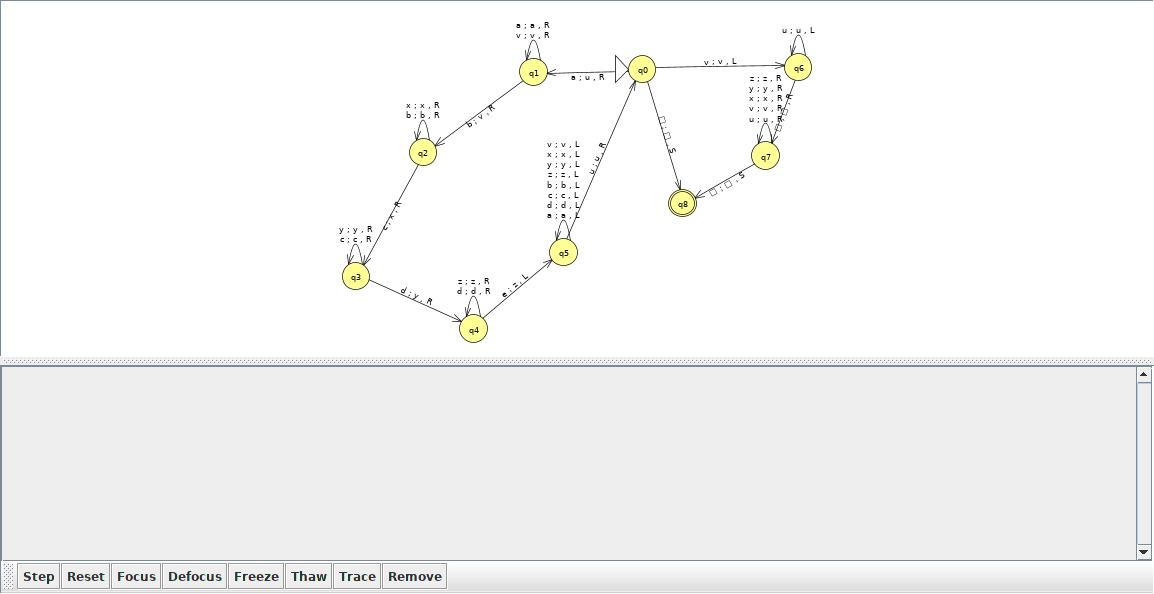
\includegraphics[width=\linewidth]{TuringMachine.jpg}
  \caption{Turing Machine}
  \label{fig:TM1}
\end{figure}
On the input string, if the tape is blank, go to the accept state. If there is an "a", mark it with a "u" and move the tape right and go to state 1. The next state skips through the rest of the "a's" and any "v's" (which are marked "b's"). It then finds a "b" on the tape and marks it with a "v". If there is no "b" it is rejected. The following states (2,3,4) do the same operation but for inputs "c,d". To transition to state 5 from state 4, the TM must find an "e" on the tape and move the head left. From this point state 5 moves the head back to the "u" which is the first marked "a" and moves the head right. At this point, the tape head should be on another "a" to mark, or on the first marked "b". If it finds an "a" it goes through the state 0-5 loop until there are no more a's to mark. If it finds a "v", then all "a's" have been marked and it moves the tape head back to the beginning of the tape with state 6. State 7 moves the tape head right across the tape for "u,v,x,y,z", if it encounters anything other than "u,v,x,y,z" it rejects. If it ends up at a blank spot on the tape, it moves to the accept state.\\

\section{Turing Machine Testing}
To test the TM, I created a shell script to generate test input strings of various lengths. It is called \path{createteststrings.sh}. It creates random strings in the language to see if any are accepted by the turing machine. The files I used for testing were \path{testfile_abcde_rand.txt} and \path{testfile_pass.txt}. I was initially hoping to find some accepted strings in my random file, but it is very difficult to match the pattern randomly. Even testing 1500 strings of various length from 5-30 characters, there weren't any acceptable strings. The second file \path{testfile_pass.txt} was used to verify known valid strings. To verify my random strings file didn't have any strings that should be accepted, I performed a grep on it to look for valid strings. I found only invalid strings and all were rejected when simulating the input strings in JFLAP.

\begin{thebibliography}{9}
\bibitem{git} 
Project github, \\\path{https://github.com/rodger79/5700-TuringMachine}
\bibitem{jflap} 
JFLAP, \\\path{http://www.jflap.org/getjflap.html}
\end{thebibliography}

\end{document}